\documentclass{my_template}
\usepackage{enumerate}
\usepackage{float}
\usepackage{graphicx}
\usepackage{amsmath}
\usepackage{geometry}
\geometry{left=2cm,right=2cm,top=2.5cm,bottom=2.8cm}
\renewcommand{\phi}{\varphi}
\renewcommand{\d}{{\rm d}}
\newcommand{\e}{\mathcal{E}}
\title{$RC$, $RL$ and $RLC$ Circuits} 
\Exercisenum{5}
\group{19}
\begin{document}
    \maketitle
    \tableofcontents
    \newpage
    \section{Introduction}
    \subsection{Transient Response of $RC$, $RL$ \& $RLC$ Series Circuit}
    \subsubsection{$RC$ Series Circuit}
    \paragraph{} Figure \ref{fig:RC} is the circuit diagram for a typical $RC$ circuit. We use a square-wave as our voltage input. When the voltage abruptly changes from 0 to $\mathcal{E}$, the voltage across the capacitor will change gradually, and the capacitor is going through the charging process.
    \begin{figure}[H]
        \centering
        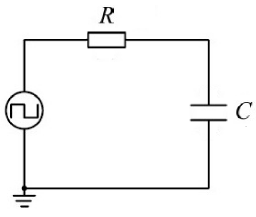
\includegraphics[width=0.5\textwidth]{fig/RC.png}
        \caption{The $RC$ Circuit}
        \label{fig:RC}
    \end{figure}
    It is determined by the following differential equation after we apply the loop rule to the circuit:
    \begin{equation}
        RC\frac{\mathrm{d}U_C}{\mathrm{d}t}+U_C=\mathcal{E},\quad U_C(0)=0.\label{eqn:RCcharging}
    \end{equation}
    The solution to this initial value problem is $$U_C=\mathcal{E}(1-e^{-\frac{t}{RC}}).$$
    \paragraph{} For the discharging process, the differential equation is 
    \begin{equation}
        RC\frac{\mathrm{d}U_C}{\mathrm{d}t}+U_C=0,\quad U_C(0)=\e.\label{eqn:RCdischarging}
    \end{equation}
    The solution is $$U_C=\e e^{-\frac{t}{RC}}.$$
    Note that in both the charging and discharging process, the voltage changes exponentially. Since $\tau=RC$ has the unit of time, it is referred to as the \emph{time constant} of the $RC$ circuit. In experiments we tend to use the \emph{half-life period} $T_{1/2}$ of the RC circuit to determined the time constant as it is easier to measure. The half-life period is the time it needs for $U_C$ to decrease to half of its initial value(during the discharging process). The relation between $\tau$ and $T_{1/2}$ are as follows: $$\tau=\frac{T_{1/2}}{\ln 2}\approx\frac{T_{1/2}}{0.693}.$$
    \subsubsection{$RL$ Series Circuit} 
    \paragraph{} The analysis of the $RL$ circuit is analogous to that of the $RC$ circuit. Here the time constant is given by $$\tau=\frac{L}{R},$$ and the relation between $\tau$ and $T_{1/2}$ stays the same.
    \subsubsection{$RLC$ Series Circuit}
    \paragraph{} After applying the loop rule to this circuit, we can get the following equation: 
    \begin{equation}
        LC\frac{\mathrm{d}^2U_C}{\mathrm{d}t^2}+RC\frac{\mathrm{d}U_C}{\mathrm{d}t}+U_C=\e, \label{eqn:RLC}
    \end{equation}
    where $U_C$ is the voltage across the capacitor. Divide both sides by $LC$ and substitute certain variables as follows: \[\beta:=\frac{R}{2L},\text{ and } \omega_0:=\frac{1}{\sqrt{LC}},\] and Equation \ref{eqn:RLC} can be transformed into 
    \begin{equation}
        \frac{\mathrm{d}^2U_C}{\mathrm{d}t^2}+2\beta\frac{\mathrm{d}U_C}{\mathrm{d}t}+\omega_0^2U_C=\omega_0^2\e.
        \label{eqn:betaandomega}
    \end{equation}
    Equation \ref{eqn:betaandomega} is mathematically equivalent to the equation of motion for an oscillating mass subject to a constant driving force and a linear drag force. The initial value for the problem is \[U_C(0)=0 \text{ and } \left.\frac{\mathrm{d}U_C}{\mathrm{d}t}\right|_{t=0}=0.\] So based on the relation between $\beta$ and $\omega_0$, there are three regimes:
    \begin{itemize}
        \item If $\beta^2-\omega_0^2<0$, the system is in the underdamped regime. The solution to the IVP is 
        \begin{equation}
            U_C=\e-\e e^{-\beta t}\left(\cos \omega t+\frac{\beta}{\omega}\sin \omega t\right),\label{eqn:under}
        \end{equation}where $\omega=\sqrt{\omega_0^2-\beta^2}$.
        \item If $\beta^2-\omega_0^2>0$, the system is in the overdamped regime. The solution to the IVP is 
        \begin{equation}
            U_C=\e-\frac{\e}{2\gamma}e^{-\beta t}[(\beta+\gamma)e^{\gamma t}-(\beta-\gamma)e^{-\gamma t}],\label{eqn:over}
        \end{equation} where $\gamma=\sqrt{\beta^2-\omega_0^2}$.
        \item If $\beta^2-\omega_0^2=0$, the system is critically damped, and 
        \begin{equation}
            U_C=\e-\e (1+\beta t)e^{-\beta t}\label{eqn:criticallydamped}
        \end{equation}
        The time constant here is $\tau=1/\beta$, which is equal to $\sqrt{LC}$.
    \end{itemize}
    \subsection{$RLC$ Resonant Circuit}
    \subsubsection{$RLC$ Series Circuit}
    \paragraph{} Figure \ref{fig:RLC} shows a generic $RLC$ series circuit. The impedance and the phase difference can be calculated with phasor technique. 
    \begin{figure}[H]
        \centering
        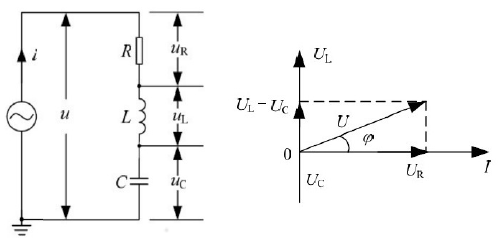
\includegraphics[width=\textwidth]{fig/RLC_Resonant.png}
        \caption{$RLC$ Series Circuit}
        \label{fig:RLC}
    \end{figure}
    Assume the current $I$ is on the real axis, the phase difference between the current and the voltages across the capacitor, the inductor and the resistance are $$\varphi_R=0,\quad \phi_C=-\frac{\pi}{2},\quad \varphi_L=\frac{\pi}{2},$$ respectively. The corresponding voltage amplitude across the elements are $$U_R=IZ=IR,\quad U_C=IZ=\frac{I}{\omega C},\quad U_L=IZ=I\omega L.$$ Therefore, the voltage amplitude is \[U=\sqrt{U_R^2+(U_L-U_C)^2},\text{ or }U=I\sqrt{R^2+\left(\omega L-\frac{1}{\omega C}\right)^2},\] and the total impedance \[Z=\sqrt{R^2+\left(\omega L-\frac{1}{\omega C}\right)^2}\] with the phase difference between the current and the voltage in the circuit 
    \begin{equation}
        \phi=\arctan\left(\frac{U_L-U_C}{U_R}\right)=\arctan\left(\frac{\omega L-\frac{1}{\omega C}}{R}\right).\label{eqn:phasedifference}
    \end{equation}
    \subsubsection{Resonance}
    \paragraph{} If the circular frequency of the voltage source satisfies the condition \[\omega_0L=\frac{1}{\omega_0C},\text{ or equivalently, }\omega_0=\frac{1}{\sqrt{LC}},\] the total impedance will reach minimum, $Z_0=R$ and the current will reach maximum. This circuit is said to be at resonance. The frequency $f_0=\frac{\omega_0}{2\pi}=\frac{1}{2\pi\sqrt{LC}}$ at which the resonance phonomenon occurs, is called the \emph{resonance frequency}.
    \vspace{-5mm}
    \paragraph{} The total impedance $Z$, the current $I$ and the phase difference $\phi=\phi_u-\phi_i$ all depend on the frequency with generic shapes of the three curves shown in Figure \ref{fig:3figures}. According to Equation \ref{eqn:phasedifference}, when the frequency is low($f<f_0$), $\phi<0$. In this situation the voltage lags behind the current and the current is said to be capacitive.
    \vspace{-5mm}
    \paragraph{} When the current is resonant($f=f_0$), the current is said to be resistive. And when the frequency is high$(f>f_0)$, the voltage leads the current and the current is said to be inductive.
    \begin{figure}[H]
        \centering
        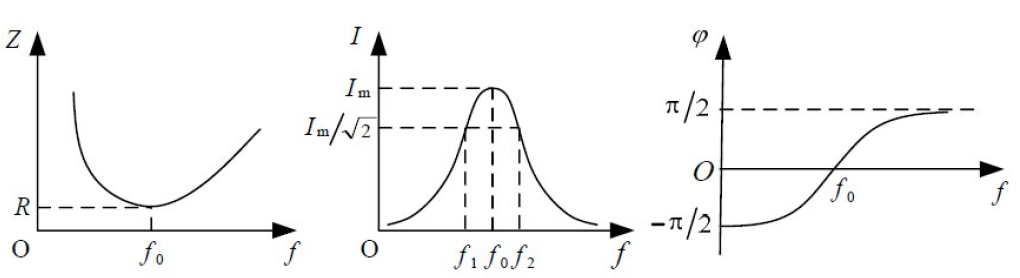
\includegraphics[width=\textwidth]{fig/3figures.png}
        \caption{The Impedance, the Current and the Phase Difference as Functions of the Frequency for a $RLC$ Series Circuit}
        \label{fig:3figures}
    \end{figure}
    \subsubsection{Quality Factor in Resonant Circuit}
    \paragraph{} When the $RLC$ circuit is at resonance, $I_m=U/R$, and the voltages across the capacitor, the resistor and the inductor are
    \begin{eqnarray*}
        U_R&=I_mR&=U,\\
        U_L&=I_mZ_L&=\frac{U}{R}\omega L\\
        U_C&=I_mZ_C&=\frac{U}{R}\frac{1}{\omega C}\\
    \end{eqnarray*}
    The quality factor is the ratio of $U_L$ and $U$: $$Q=\frac{U_L}{U}=\frac{\omega_0L}{R}=\frac{1}{\omega_0RC}=\frac{\sqrt{LC}}{RC}.$$When the total voltage is fixed, the greater $Q$ is, the greater $U_L$ and $U_C$ are. The value of $Q$ can be used to quantify the efficiency of resonant circuits.
    \vspace{-5mm}
    \paragraph{}The quality factor can also be found as $$Q=\frac{f_0}{f_1-f_2},$$ where $f_1$ and $f_2$ are two frequencies such that $I(f_1)=I(f_2)=I_m/\sqrt{2}.$
    \section{Apparatus \& Measurement Procedure}
    \subsection{Apparatus}
    \paragraph{}The measurement setup consists of the following main elements: a signal generator, an oscilloscope, a wiring board, a fixed resistor 100$\Omega$, a variable resistor 2k$\Omega$, a capacitor 0.1 $\mu$F and an inductor (10 mH). The uncertainty of the apparatus is listed in Table \ref{tab:apparatus}. 
    \begin{table}[H]
        \centering
        \begin{tabular}{|c|c|}
            \hline
            Apparatus&Uncertainty\\\hline
            multimeter(Ohm)&0.01[$\Omega$]\\\hline
            multimeter(capacitance)&0.01[nF]\\\hline
            oscilloscope($U$)&0.01[V]\\\hline
            oscilloscope($\Delta t$)&0.01[$\mu$s] or 0.001[$\mu$s]\\\hline
            function generator(frequency)&0.001[Hz]\\\hline
            function generator(amplitude)&0.001[V$_{\rm pp}$]\\\hline
        \end{tabular}
        \caption{The Uncertainty of the Measurement in Lab}
        \label{tab:apparatus}
    \end{table}
    \subsection{Measurement Procedure}
    \subsubsection{$RC$, $RL$ Circuit}
    \begin{enumerate}
        \item  I first measured the resistance of the fixed resistor and the capacitance of the capacitor using two multimeters.
        \item I connected the fixed resistor and the capacitor in series and set the channel 1 of the oscilloscope to measure the input voltage, and channel 2 to measure the voltage across the capacitor. I made sure that all ground lines were in the same node and only turned on the function generator after the whole circuit was set up. 
        \item I chose the square wave function on the function generator and adjusted its frequency so that the capacitor could make a full charging/ discharging process. Then I took a photo of the waveform and used ``cursor" on the oscilloscope to measure the half life period.\label{enum:2}
        \item I replaced the capacitor with the inductor, and used channel 2 to measure the voltage across the resistor. Then I repeated step \ref{enum:2}.
    \end{enumerate}
    \subsubsection{$RLC$ Series Circuit}
    \begin{enumerate}
        \item I connected the variable resistor, the capacitor and the inductor in series, and let channel 1 measure the input voltage and channel 2 measure the voltage across the capacitor. I chose the square wave on the function generator and adjusted its frequency so that the capacitor could make a full charging/ discharging process. I adjusted the resistance of the variable resistor so that the circuit was in overdamped, underdamped and critically damped regimes. I took photoes of the oscilloscope for each of the regime.
        \item For critically damped circuit, I measured the half-life period. 
    \end{enumerate}
    \subsubsection{$RLC$ Resonant Circuit}
    \begin{enumerate}
        \item I replaced the variable resistor with the fixed resistor and used the sine wave function on the function generator. I made sure that channel 2 measured the voltage across the resistor. Then I changed the value of the frequency of the input voltage and recorded the corresponding value of the voltage amplitude across the resistor($U_R$). I recorded 25 sets of data and determined the resonant frequency by finding the largest $U_R$. 
    \end{enumerate}
    \section{Result}
    \subsection{The Transient Response of $RC$ Circuit}\label{sec:RC}
    \paragraph{} Table \ref{tab:RC} shows the original data for the $RC$ circuit and Figure \ref{fig:RCresponse} is the image on the oscilloscope. The theoretical time constant is given by \[\tau_{\rm theoretical}=RC=99.96\times 102.60\times 10^{-9}=1.026\times 10^{-5}[\rm s]=10.26[\mu s]\pm 0.10[\mu s].\]
    \begin{table}[H]
        \begin{center}
            $\e$: 4.000[V$_{\rm pp}]\pm 0.001 [V_{pp}$]
            \begin{tabular}{|c|c|c|c|}
                \hline
                $R[\Omega]\pm 0.01[\Omega]$&99.96&$f[\rm kHz]\pm 0.001[Hz]$&1.000000\\\hline
                $C[\rm nF]\pm 0.01[nF]$&102.60&$T_{1/2}[\rm \mu s]\pm 0.001[\mu s]$&7.200\\\hline
            \end{tabular}
        \end{center}
        \caption{The Original Data for $RC$ Circuit}
        \label{tab:RC}
    \end{table}
    \begin{figure}[H]
        \centering
        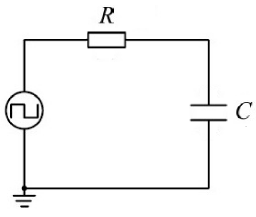
\includegraphics[width=\textwidth]{fig/RC.jpg}
        \caption{The Transient Response of $RC$ Circuit}
        \label{fig:RCresponse}
    \end{figure}
    \paragraph{}The experimental time constant is given by \[\tau_{\rm experimental}=\frac{T_{1/2}}{\ln 2}=\frac{7.2}{0.693}=10.3874[\mu \rm s]\pm 0.0014[\mu s].\]
    \subsection{The Transient Response of $RL$ Circuit}\label{sec:RL}
    \paragraph{} Table \ref{tab:RL} is the original data for the $RL$ circuit we use in lab, and Figure \ref{fig:RLresponse} is the image on the oscilloscope of the transient response of the $RL$ circuit. The theoretical time constant is given by $$\tau_{\rm theoretical}=\frac{L}{R}=\frac{0.01}{99.96}=100.040[\mu \rm s]\pm 0.010[\mu s].$$
    \begin{table}[H]
        \begin{center}
            $\e$: 4.000[V$_{\rm pp}]\pm 0.001 [V_{pp}$]
            \begin{tabular}{|c|c|c|c|}
                \hline
                $R[\Omega]\pm 0.01[\Omega]$&99.96&$f[\rm kHz]\pm 0.001[Hz]$&1.000000\\\hline
                $L[\rm H]\pm 0[H]$&0.01&$T_{1/2}[\rm \mu s]\pm 0.01[\mu s]$&80.00\\\hline
            \end{tabular}
        \end{center}
        \caption{The Original Data for $RL$ Circuit}
        \label{tab:RL}
    \end{table}
    \begin{figure}[H]
        \centering
        \includegraphics[width=\textwidth]{fig/RL.jpg}
        \caption{The Transient Response of $RL$ Circuit}
        \label{fig:RLresponse}
    \end{figure}
    The experimental value is also given by \[\tau_{\rm experimental}=\frac{T_{1/2}}{\ln 2}=\frac{80}{\ln 2}=115.416[\mu \rm s]\pm 0.014[\mu s]\]
    \subsection{The $RLC$ Damped Circuit}
    \subsubsection{Critically Damped Circuit}\label{sec:RLC}
    \paragraph{} Table \ref{tab:RLC damped} shows the data for the critically damped $RLC$ circuit and Figure \ref{fig:RLCcritical} is the image on the oscilloscope. The theoretical time constant is given as $$\tau_{\rm theoretical}=\sqrt{LC}=\sqrt{0.01\times 102.60\times 10^{-9}}[\rm s]=32.0312[\mu s]\pm 0.0016[\mu s].$$
    \begin{table}[H]
        \begin{center}
            $\e$: 4.000[V$_{\rm pp}]\pm 0.001 [V_{pp}$]
            \begin{tabular}{|c|c|c|c|}
                \hline
                $C[\rm nF]\pm 0.01[nF]$&102.60&$f[\rm kHz]\pm 0.001[Hz]$&1.000000\\\hline
                $L[\rm H]\pm 0[H]$&0.01&$T_{1/2}[\rm \mu s]\pm 0.01[\mu s]$&60.00\\\hline
            \end{tabular}
        \end{center}
        \caption{The Original Data for $RLC$ Circuit When It is Critically Damped}
        \label{tab:RLC damped}
    \end{table}
    \begin{figure}[H]
        \centering
        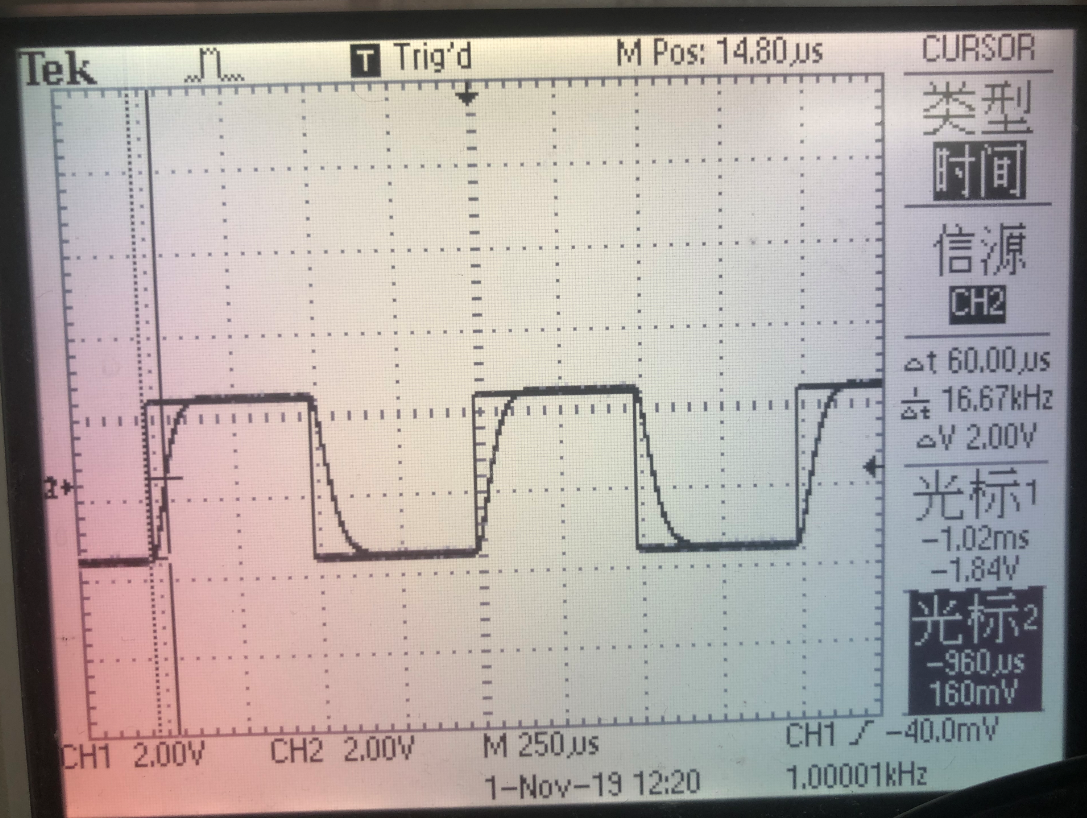
\includegraphics[width=\textwidth]{fig/critically.png}
        \caption{The Critically Damped $RLC$ Circuit}
        \label{fig:RLCcritical}
    \end{figure}
    The experimental time constant is $$\tau_{\rm experimental}=\frac{T_{1/2}}{1.68}=\frac{60}{1.68}=35.714[\rm\mu s]\pm 0.006[\mu s].$$
    \subsubsection{Underdamped and Overdamped Regimes}
    \paragraph{} Figure \ref{fig:RLCunder} shows the image on the oscilloscope of the underdamped regime of the $RLC$ circuit and Figure \ref{fig:RLCover} is the overdamped regime.
    \begin{figure}[H]
        \centering
        \includegraphics[width=\textwidth]{fig/under.jpg}
        \caption{The Underdamped Regime of the $RLC$ Circuit}
        \label{fig:RLCunder}
    \end{figure}
    \begin{figure}[H]
        \centering
        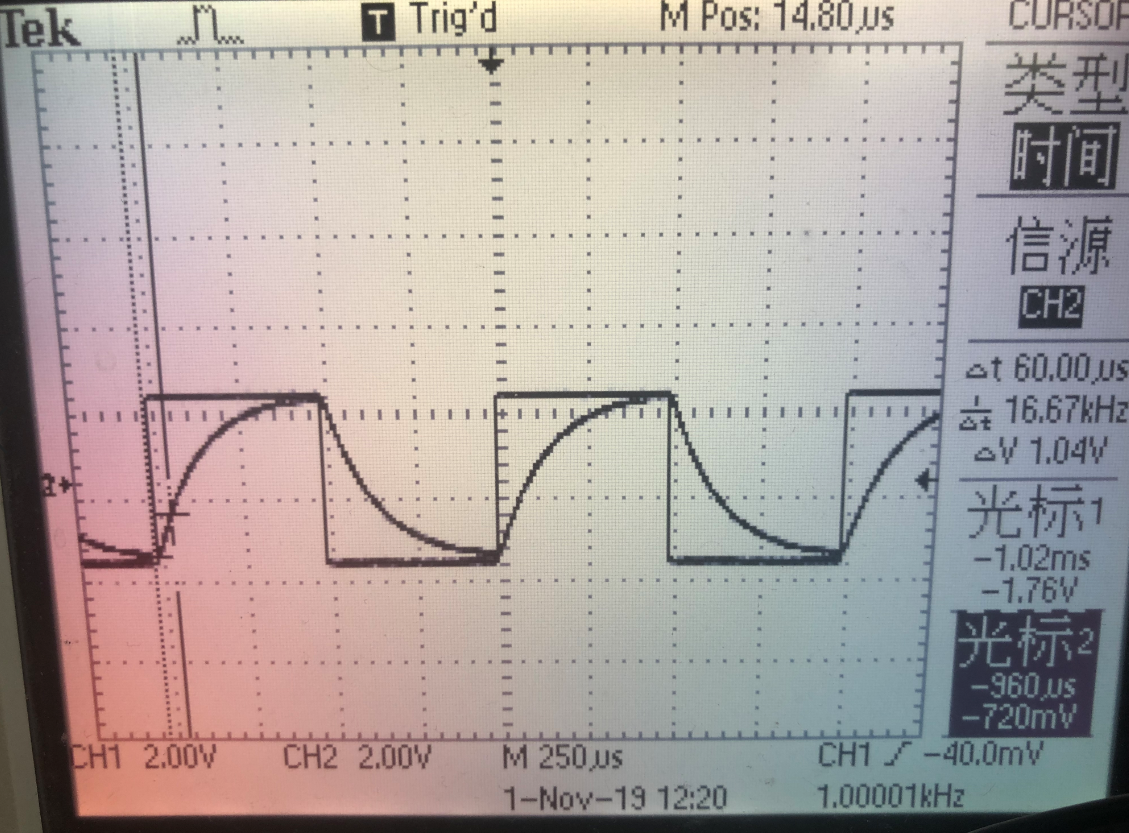
\includegraphics[width=\textwidth]{fig/overdamped.jpg}
        \caption{The Overdamped Regime of the $RLC$ Circuit}
        \label{fig:RLCover}
    \end{figure}
    \subsection{$RLC$ Resonant Circuit}\label{sec:RLCResonant}
    \paragraph{} Table \ref{tab:RLC Resonant} is the original data for this section. I chose the resonant frequency $f_0=5050[\rm Hz]$, and used these data to plot three graphs: $\frac{I}{I_m}$ vs. $\frac{f}{f_0}$, $\phi_{\rm theoretical}$ vs. $\frac{f}{f_0}$ and $\phi_{\rm experimental}$ vs. $\frac{f}{f_0}$.
    \begin{table}[H]
        \centering
        \begin{tabular}{|c|c|c|}
            \hline
            \multicolumn{3}{|c|}{$R$: 99.96$[\Omega]\pm 0.01[\Omega]$, $L: 0.01\rm [H]\pm 0[H]$, $C: 102.60\rm [nF]\pm 0.01[nF]$}\\\hline
            \multicolumn{3}{|c|}{$f_0: 5050.000[\rm Hz]\pm 0.001[Hz]$, $\e: 4.000[\rm V_{pp}]\pm 0.001[V_{pp}]$}\\\hline
            &$U_R[\rm V]\pm 0.01[V]$&$f\rm[Hz]\pm 0.001[Hz]$\\\hline
            1&1.12&3000.000\\\hline
            2&1.60&3500.000\\\hline
            3&2.32&4000.000\\\hline
            4&2.72&4220.000\\\hline
            5&2.88&4300.000\\\hline
            6&3.44&4600.000\\\hline
            7&3.52&4700.000\\\hline
            8&3.68&4800.000\\\hline
            9&3.76&4900.000\\\hline
            10&3.84&5000.000\\\hline
            11&3.84&5050.000\\\hline
            12&3.84&5080.000\\\hline
            13&3.84&5100.000\\\hline
            14&3.76&5150.000\\\hline
            15&3.68&5200.000\\\hline
            16&3.60&5300.000\\\hline
            17&3.44&5400.000\\\hline
            18&3.36&5500.000\\\hline
            19&3.20&5600.000\\\hline
            20&2.88&5800.000\\\hline
            21&2.72&5930.000\\\hline
            22&2.48&6100.000\\\hline
            23&2.08&6500.000\\\hline
            24&1.76&7000.000\\\hline
            25&1.28&8000.000\\\hline
        \end{tabular}
        \caption{The Original Data for the $RLC$ Resonant Circuit}
        \label{tab:RLC Resonant}
    \end{table}
    \vspace{-5mm}
    \paragraph{} The theoretical resonant frequency is given in the following equation$${f_0}_t=\frac{1}{2\pi\sqrt{LC}}.$$ In our lab, $L=0.01[\rm H]$, $C=102.60[\rm nF]$, so the resonant frequency is $${f_0}_t=\frac{1}{2\times\pi\times\sqrt{0.01\times 102.60\times 10^{-9}}}=4968.7[\rm Hz]\pm 0.2[Hz].$$
    \paragraph{} As for the experimental resonant frequency, I chose the frequency corresponding to the largest $U_R$: $${f_0}_e=5050.000[\rm Hz]\pm 0.001[Hz].$$
    \paragraph{} Table \ref{tab:Iandf} are the data after manipulation to study the relation between amplitude and frequency. Since for a fixed resistor, the voltage amplitude and the current amplitude is of direct proportionality, we can conclude that $I/I_m=U/U_m$. For example, when $U=1.12[\rm V]$, $U_m=3.84[\rm V]$, $f=3000[\rm V]$, $f_0=5050[\rm V]$, 
    \begin{equation*}
        \begin{split}
            \frac{I}{I_m}=\frac{U}{U_m}=\frac{1.12}{3.84}=0.292\pm 0.003\\
            \frac{f}{f_0}=\frac{3000}{5050}=0.5940594\pm 0.0000002\\
        \end{split}
    \end{equation*}
    \begin{table}[H]
        \begin{center}
            \begin{tabular}{|c|c|c|c|c|}
                \hline
                &$\frac{I}{I_m}$&Uncertainty&\(\frac{f}{f_0}\)&Uncertainty\\\hline
                1&0.292&0.003&0.5940594&0.0000002\\\hline
                2&0.417&0.003&0.6903693&0.0000002\\\hline
                3&0.604&0.003&0.7920792&0.0000003\\\hline
                4&0.708&0.003&0.8356436&0.0000003\\\hline
                5&0.750&0.003&0.8514851&0.0000003\\\hline
                6&0.896&0.003&0.9108911&0.0000003\\\hline
                7&0.917&0.003&0.9306931&0.0000003\\\hline
                8&0.958&0.003&0.9504951&0.0000003\\\hline
                9&0.979&0.003&0.9702970&0.0000003\\\hline
                10&1.000&0.003&0.9900990&0.0000003\\\hline
                11&1.000&0.003&1.0000000&0.0000003\\\hline
                12&1.000&0.003&1.0059406&0.0000003\\\hline
                13&1.000&0.003&1.0099010&0.0000003\\\hline
                14&0.979&0.003&1.0198020&0.0000003\\\hline
                15&0.958&0.003&1.0297030&0.0000003\\\hline
                16&0.938&0.003&1.0495050&0.0000003\\\hline
                17&0.896&0.003&1.0693070&0.0000003\\\hline
                18&0.875&0.003&1.0891089&0.0000003\\\hline
                19&0.833&0.003&1.1089109&0.0000003\\\hline
                20&0.750&0.003&1.1485149&0.0000003\\\hline
                21&0.708&0.003&1.1742574&0.0000003\\\hline
                22&0.656&0.003&1.1207921&0.0000003\\\hline
                23&0.542&0.003&1.2871287&0.0000003\\\hline
                24&0.458&0.003&1.3861386&0.0000003\\\hline
                25&0.333&0.003&1.5841584&0.0000004\\\hline
            \end{tabular}
        \end{center}
        \caption{The Amplitude in Frequency Domain}
        \label{tab:Iandf}
    \end{table}
    \begin{figure}[H]
        \centering
        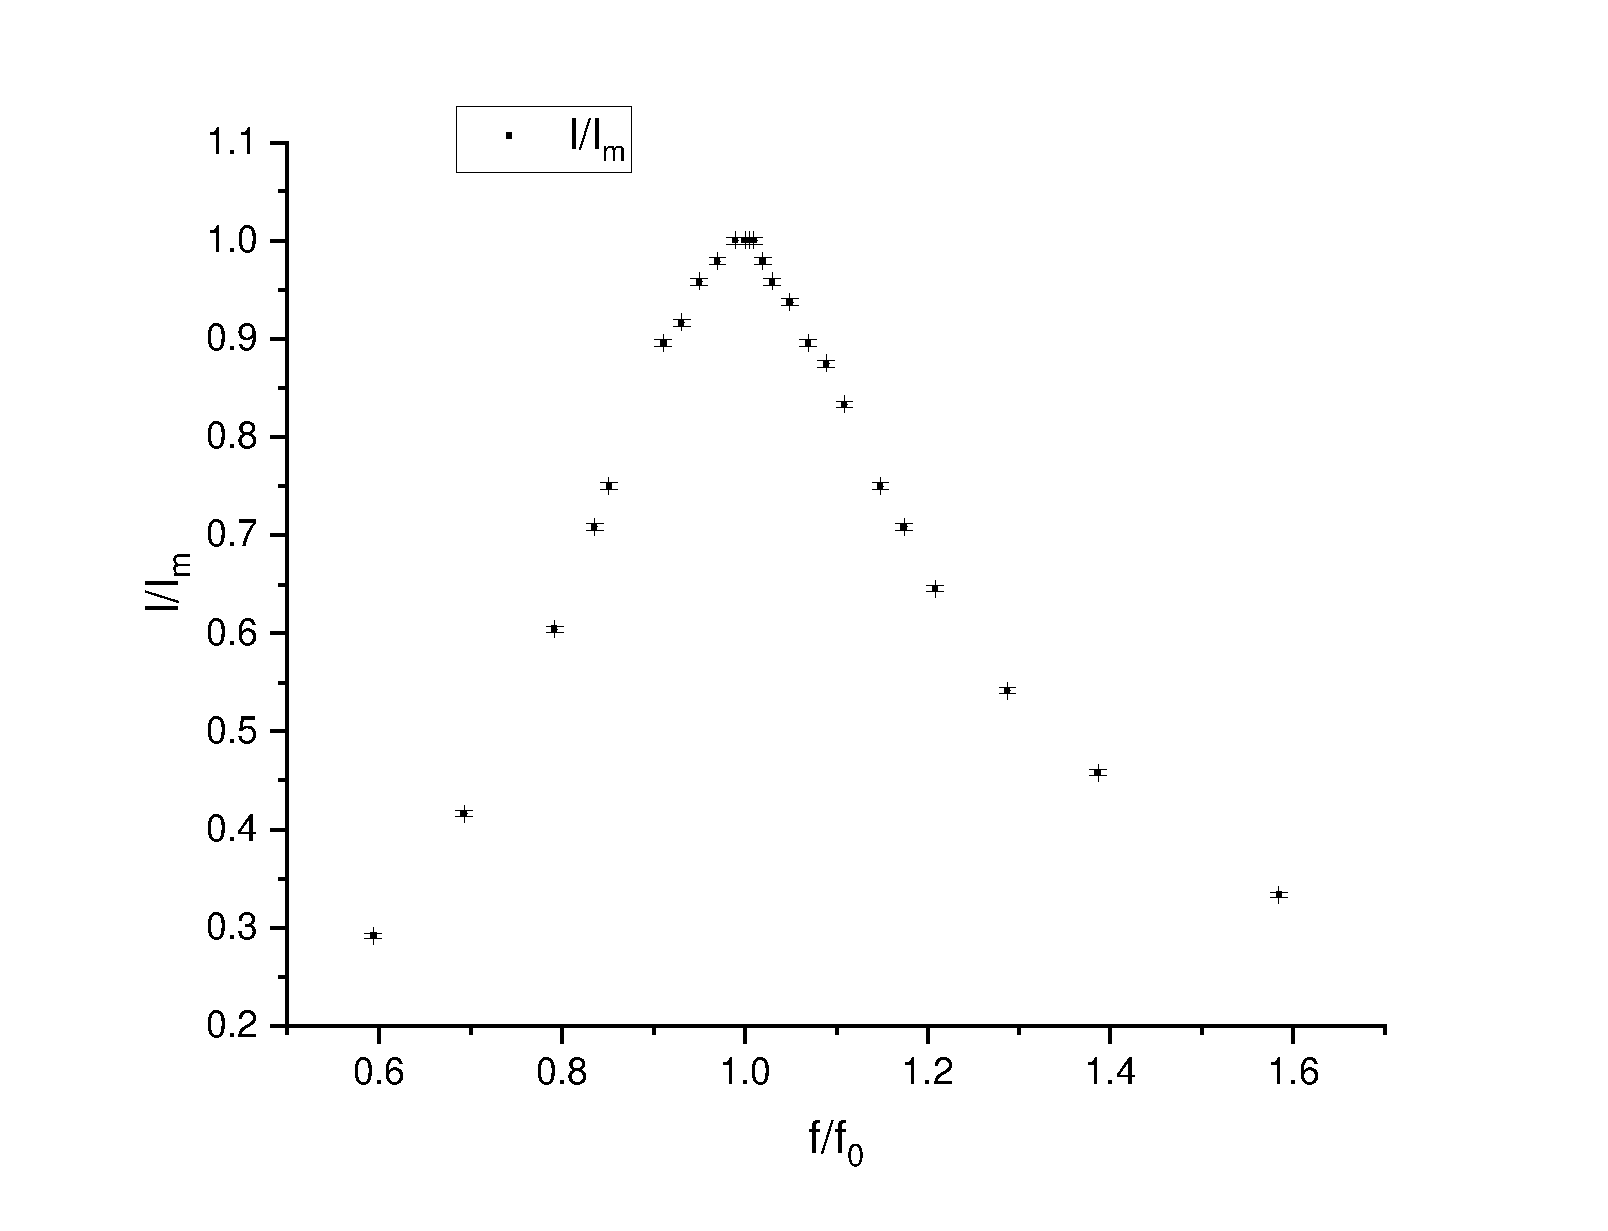
\includegraphics[width=\textwidth]{fig/Iandf.pdf}
        \caption{The Relation of $I/I_m$ vs. $f/f_0$}
        \label{fig:Iandf}
    \end{figure}
    \paragraph{} As for the phase difference, the theoretical value is given by Equation \ref{eqn:phasedifference}, $$\phi=\arctan\left(\frac{\omega L-\frac{1}{\omega C}}{R}\right).$$ For example, when $f=3000[\rm Hz]$, $u_f=0.001[\rm Hz]$, $\omega=2\pi f=18849.556[\rm Hz]$, $L=0.01[\rm H]$, $C=102.60[\rm nF]$, $R=99.96[\Omega]$, then 
    \begin{equation*}
        \begin{split}
            \phi&=\arctan\left(\frac{18849.556\times 0.01-\frac{1}{18849.556\times 102.60\times 10^{-9}}}{99.96}\right)\\
            &=-1.27547[\rm rad]\pm 0.00002[rad]
        \end{split}
    \end{equation*}
    Table \ref{tab:phit} shows the results of the calculations above and I used them to plot Figure \ref{fig:phit}.
    \begin{table}
        \centering
        \begin{tabular}{|c|c|c|c|c|}
            \hline
            &$\phi_t$[rad]&Uncertainty[rad]&$\frac{f}{f_0}$&Uncertainty\\\hline
            1&-1.27547&0.00002&0.5940594&0.0000002\\\hline
            2&-1.14989&0.00005&0.6903693&0.0000002\\\hline
            3&-0.93863&0.00010&0.7920792&0.0000003\\\hline
            4&-0.79763&0.00014&0.8356436&0.0000003\\\hline
            5&-0.73616&0.00017&0.8514851&0.0000003\\\hline
            6&-0.4493&0.0002&0.9108911&0.0000003\\\hline
            7&-0.3345&0.0003&0.9306931&0.0000003\\\hline
            8&-0.2125&0.0003&0.9504951&0.0000003\\\hline
            9&-0.0868&0.0003&0.9702970&0.0000003\\\hline
            10&0.0392&0.0003&0.9900990&0.0000003\\\hline
            11&0.1010&0.0003&1.0000000&0.0000003\\\hline
            12&0.1375&0.0003&1.0059406&0.0000003\\\hline
            13&0.1615&0.0003&1.0099010&0.0000003\\\hline
            14&0.2202&0.0003&1.0198020&0.0000003\\\hline
            15&0.2770&0.0003&1.0297030&0.0000003\\\hline
            16&0.3835&0.0003&1.0495050&0.0000003\\\hline
            17&0.4799&0.0002&1.0693070&0.0000003\\\hline
            18&0.5662&0.0002&1.0891089&0.0000003\\\hline
            19&0.6428&0.0002&1.1089109&0.0000003\\\hline
            20&0.77023&0.00016&1.1485149&0.0000003\\\hline
            21&0.83770&0.00014&1.1742574&0.0000003\\\hline
            22&0.91147&0.00012&1.1207921&0.0000003\\\hline
            23&1.03862&0.00008&1.2871287&0.0000003\\\hline
            24&1.14125&0.00005&1.3861386&0.0000003\\\hline
            25&1.25769&0.00003&1.5841584&0.0000004\\\hline
        \end{tabular}
        \caption{The Relation of the Theoretical Phase Difference in Frequency Domain}
        \label{tab:phit}
    \end{table}
    \begin{figure}[H]
        \centering
        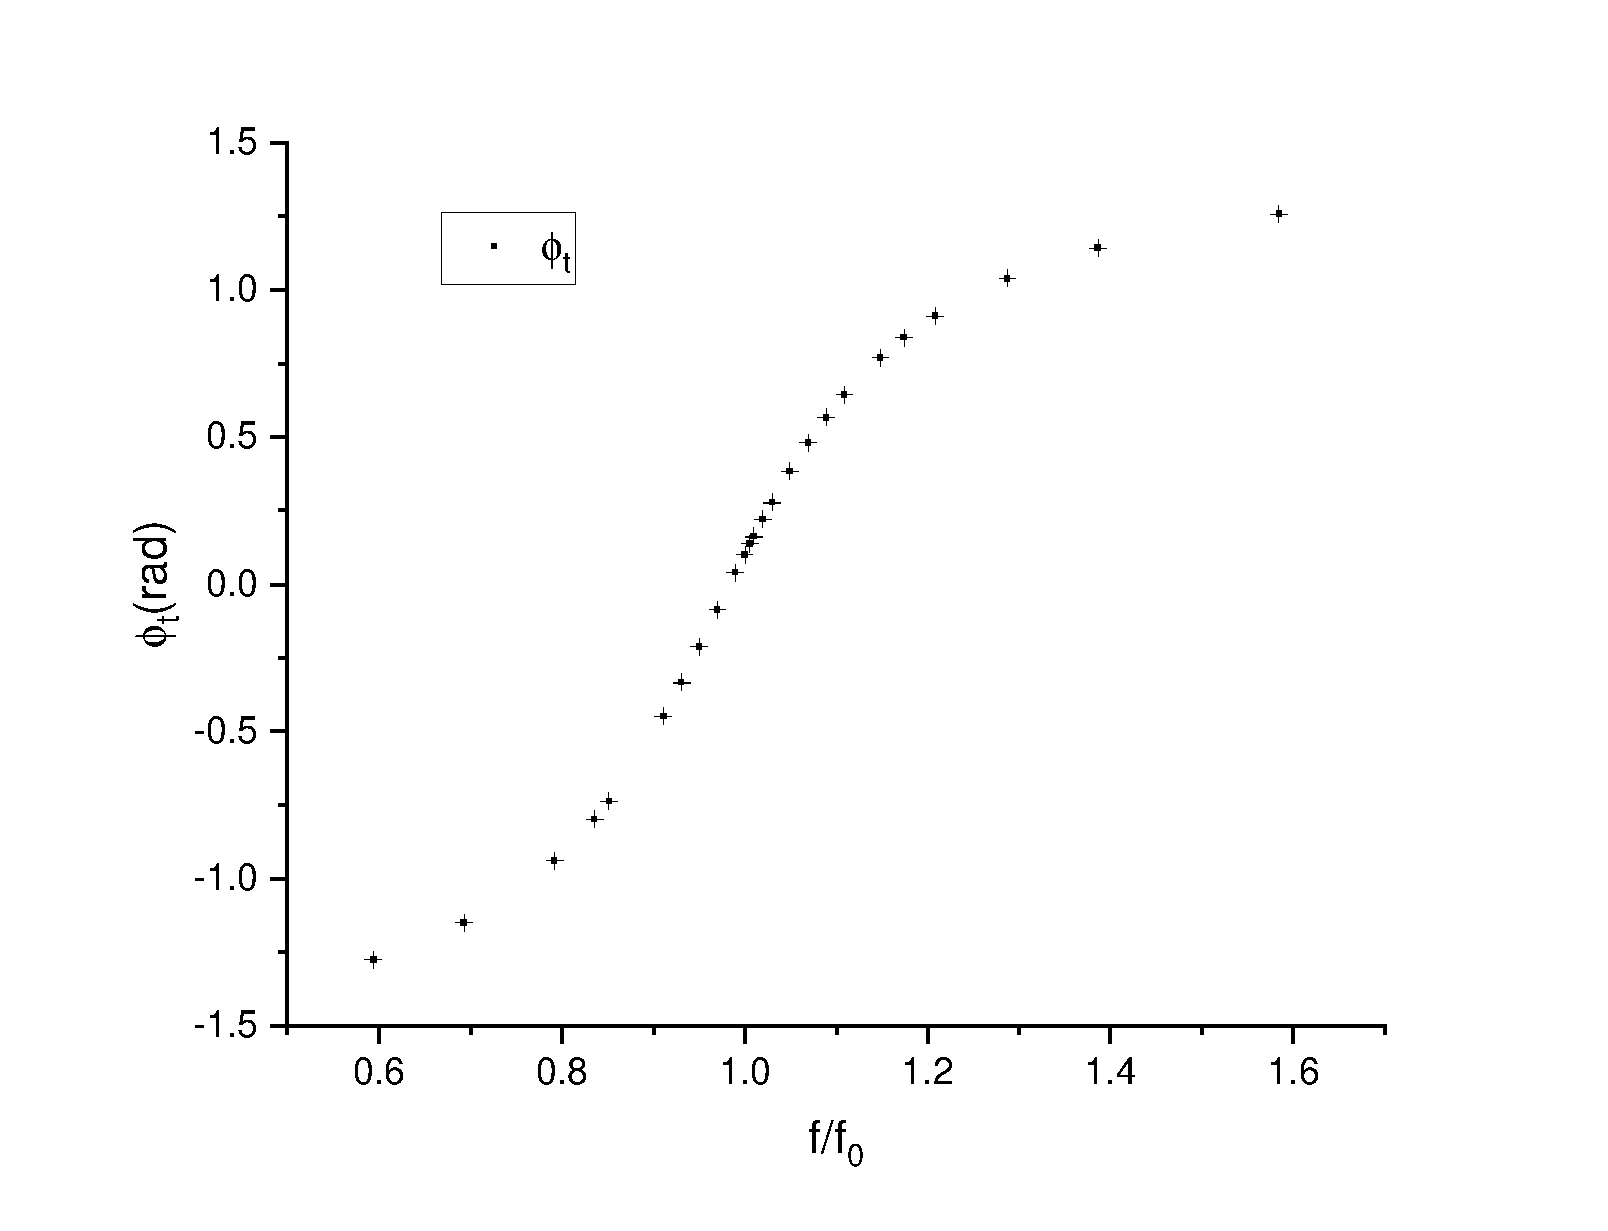
\includegraphics[width=\textwidth]{fig/phit.pdf}
        \caption{The Theoretical Phase Difference $\phi$ vs. $f/f_0$}
        \label{fig:phit}
    \end{figure}
    \paragraph{}The experimental phase difference is given as $$\phi={\rm sgn}\left(\frac{f}{f_0}-1\right)\arccos\left(\frac{U_R}{U_m}\right),$$ where the sign function is defined as 
    $${\rm sgn}x=
    \left\{\begin{array}{c}
        \frac{x}{|x|},\text{if }x\not=0\\
        0,\text{if }x=0
    \end{array}\right..$$
    For example, when $f=3000[\rm Hz]$, $f_0=5050[\rm Hz]$, $U_R=1.12[\rm Hz]$, $U_m=3.84[\rm Hz]$, $$\phi={\rm sgn}\left(\frac{3000}{5050}-1\right)\arccos\left(\frac{1.12}{3.84}\right)=-1.275[\rm rad]\pm 0.003[rad].$$
    The results are listed in Table \ref{tab:phie}, and I have plotted Figure \ref{fig:phie}.
    \begin{table}[H]
        \begin{center}
            \begin{tabular}{|c|c|c|c|c|}
                \hline
                &$\phi_e$[rad]&Uncertainty[rad]&$\frac{f}{f_0}$&Uncertainty\\\hline
                1&-1.275&0.003&0.5940594&0.0000002\\\hline
                2&-1.141&0.003&0.6903693&0.0000002\\\hline
                3&-0.922&0.004&0.7920792&0.0000003\\\hline
                4&-0.784&0.005&0.8356436&0.0000003\\\hline
                5&-0.723&0.005&0.8514851&0.0000003\\\hline
                6&-0.460&0.008&0.9108911&0.0000003\\\hline
                7&-0.411&0.009&0.9306931&0.0000003\\\hline
                8&-0.290&0.013&0.9504951&0.0000003\\\hline
                9&-0.204&0.018&0.9702970&0.0000003\\\hline
                10&0&0$^\star$&0.9900990&0.0000003\\\hline
                11&0&0&1.0000000&0.0000003\\\hline
                12&0&0&1.0059406&0.0000003\\\hline
                13&0&0&1.0099010&0.0000003\\\hline
                14&0.204&0.018&1.0198020&0.0000003\\\hline
                15&0.290&0.013&1.0297030&0.0000003\\\hline
                16&0.355&0.010&1.0495050&0.0000003\\\hline
                17&0.460&0.008&1.0693070&0.0000003\\\hline
                18&0.505&0.007&1.0891089&0.0000003\\\hline
                19&0.586&0.006&1.1089109&0.0000003\\\hline
                20&0.723&0.005&1.1485149&0.0000003\\\hline
                21&0.784&0.005&1.1742574&0.0000003\\\hline
                22&0.869&0.004&1.1207921&0.0000003\\\hline
                23&0.998&0.004&1.2871287&0.0000003\\\hline
                24&1.095&0.003&1.3861386&0.0000003\\\hline
                25&1.231&0.003&1.5841584&0.0000004\\\hline
            \end{tabular}
        \end{center}
        \caption{The Relation of the Experimental Phase Difference in Frequency Domain}
        $^\star$ The uncertainty calculated based on the formula given in Section \ref{sec:u} is infinity(including the three data below), but since here $U_R/U_m$ must be 1 as I chose the largest $U_R$ as the value of $U_m$, it makes no sense that the uncertainty is infinity. So, I ``make'' the uncertainty zero here.         
        \label{tab:phie}
    \end{table}
    \begin{figure}[H]
        \centering
        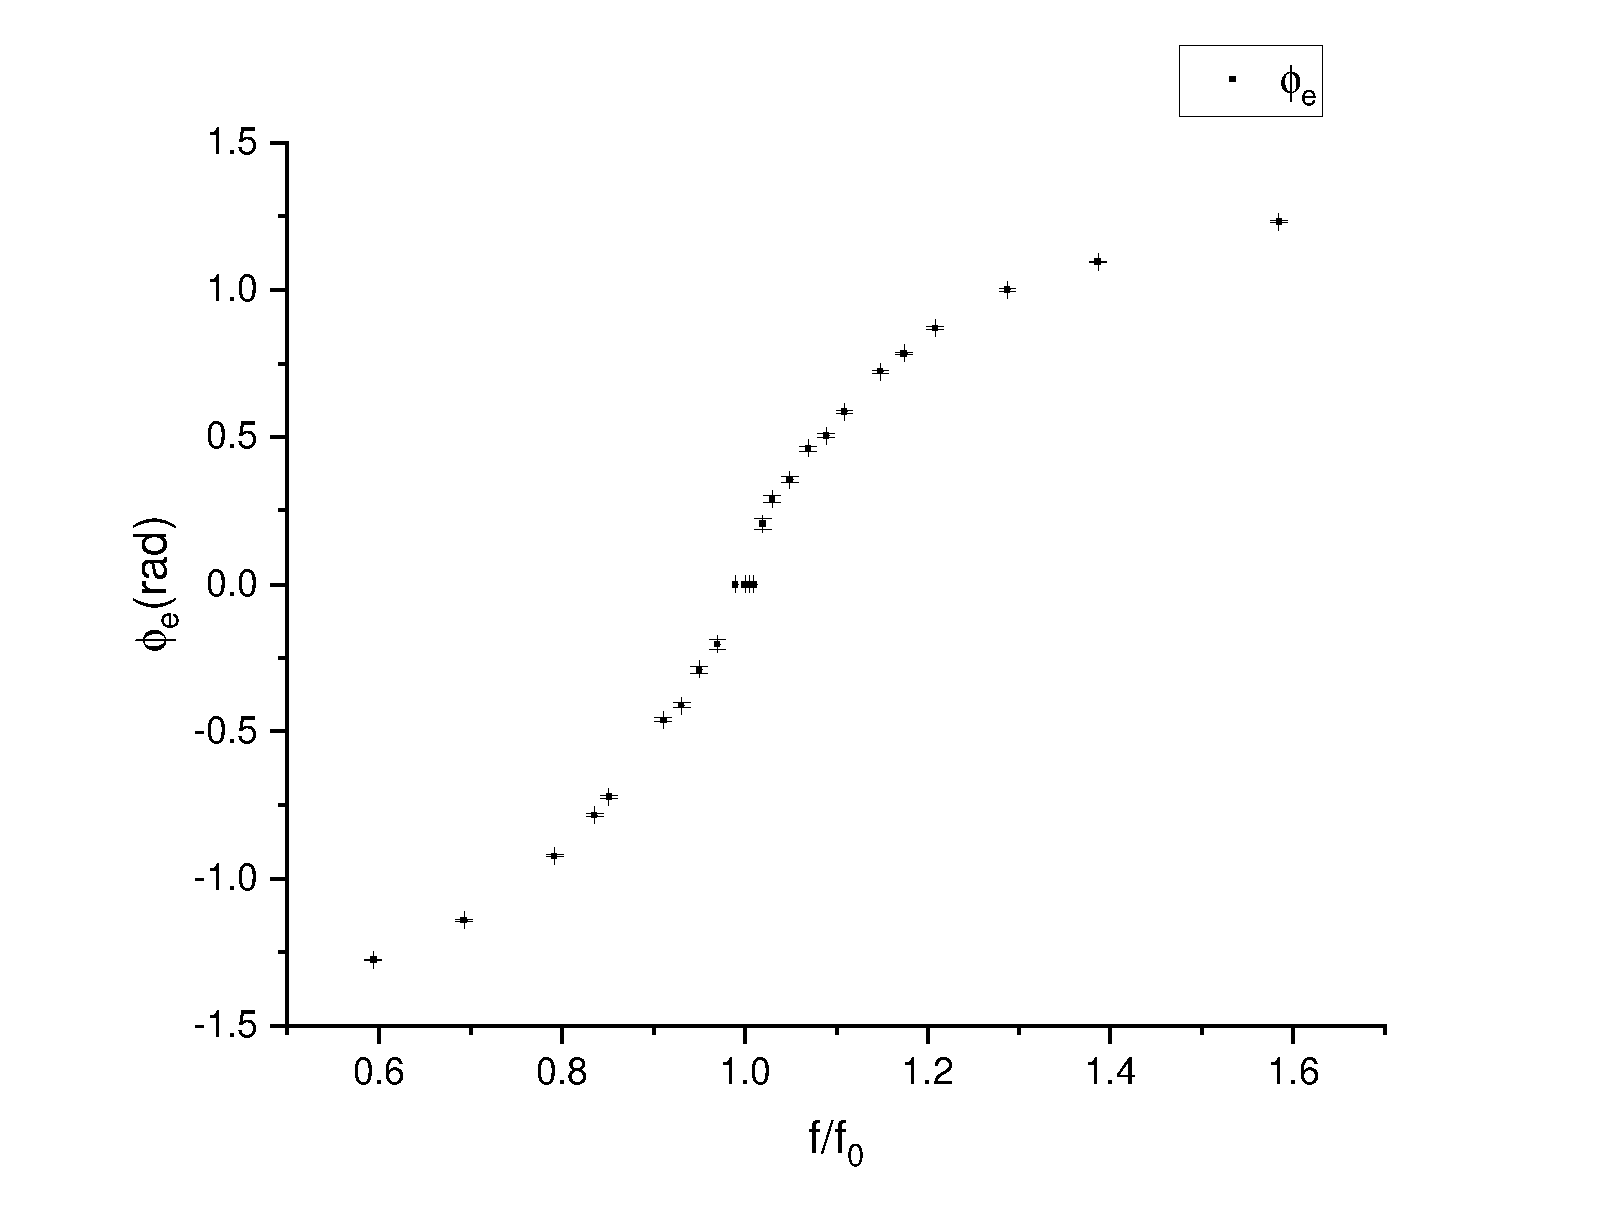
\includegraphics[width=\textwidth]{fig/phie.pdf}
        \caption{The Experimental Phase Difference $\phi$ vs. $f/f_0$}
        \label{fig:phie}
    \end{figure}
    \paragraph{}The theoretical quality factor is given by $$Q=\frac{\sqrt{LC}}{RC}.$$ In our circuit, $L=0.01[\rm H]$, $C=102.60[\rm nF]$, $R=99.96[\Omega]$. So, $$Q_t=\frac{\sqrt{0.01\times 102.60\times 10^{-9}}}{99.96\times 102.60\times 10^{-9}}=3.1232\pm 0.0003.$$
    \vspace{-5mm} 
    \paragraph{}The experimental quality factor is $$Q=\frac{f_0}{f_2-f_1}.$$ Since $\frac{U_m}{\sqrt{2}}=\frac{3.84}{\sqrt2}\approx 2.72[\rm V]$, from Table \ref{tab:RLC Resonant}, we can see that $f_2=5930[\rm Hz]$ and $f_1=4220[\rm Hz]$. Therefore, the experimental quality factor is $$Q_e=\frac{5050}{5930-4220}=2.9532164\pm 0.0000006.$$
    \section{Discussion}
    \subsection{The Transient Response of $RC$ Circuit}
    \paragraph{} As shown in Figure \ref{fig:RCresponse}, when the input voltage changes abruptly, the voltage across the capacitor will not suddenly change. Instead, it will experience exponential saturation until it reaches the input voltage. And the steady state is the same as we analyze the circuit. As the capacitor can be view as an open circuit is DC circuit, the voltage across it must be the source voltage.
    \vspace{-5mm} 
    \paragraph{} The theoretical and experimental time constant are listed as follows:
    \begin{eqnarray*}
        \tau_{\rm theoretical}&=10.26[\mu s]\pm 0.10[\mu s]\\
        \tau_{\rm experimental}&=10.3874[\mu \rm s]\pm 0.0014[\mu s].
    \end{eqnarray*}
    As we can see, they are the same in principle. The minor deviation may comes from the inaccuracy of the oscilloscope. I have noticed that the change of the time interval and the voltage on the oscilloscope is not continuous. Therefore, although it is said that the uncertainty of the half-life period is $0.01[\mu$s], the actual uncertainty will be greater. By counting this factor, I assume my measurement is valid and the theoretical and the experimental time constants coincide with each other. 
    \subsection{The Transient Response of $RL$ Circuit}
    \paragraph{} As shown in Figure \ref{fig:RLresponse}, when the input voltage changes abruptly, the voltage across the resistor in the $RL$ circuit will not suddenly change. As the current is directly proportional to this voltage, we may conclude that the current in this circuit will experience exponential saturation. For the steady state, the voltage across the resistor will eventually be equal to the source voltage because the inductor is considered to be of resistance 0 in a DC circuit. 
    \vspace{-5mm}
    \paragraph{}The theoretical and experimental time constant are listed as follows:
    \begin{eqnarray*}
        \tau_{\rm theoretical}&=100.040[\mu \rm s]\pm 0.010[\mu s]\\
        \tau_{\rm experimental}&=115.416[\mu \rm s]\pm 0.014[\mu s].\\
    \end{eqnarray*}
    So the theoretical and the experimental data is not quite close this time. Besides the uncertainty caused by the oscilloscope, there is another reason for it. We did not measure the actual inductance of the coil. Instead, we directly use the inductance labelled on it(0.01H), and we did not even account for the uncertainty of it(we assume $u_L=0$). The actual inductance might vary due to temperature and possibly other factors, and in our case, is lower than the inductance on the label.
    \subsection{The Transient Response of $RLC$ Circuit}
    \paragraph{} When the circuit is critically damped, the time constants are listed below:
    \begin{eqnarray*}
        \tau_{\rm theoretical}&=32.0312[\mu s]\pm 0.0016[\mu s]\\
        \tau_{\rm experimental}&=35.714[\rm\mu s]\pm 0.006[\mu s]\\
    \end{eqnarray*}
    These two time constants are quite close to each other, so after taking the uncertainty of the oscilloscope into consideration, we can conclude that these two time constants are identical. 
    \vspace{-5mm}
    \paragraph{} When the circuit is underdamped, the voltage across the capacitor will oscillate before going to stability(Figure \ref{fig:RLCunder}). The oscillation is due to the trigonometric part in Equation \ref{eqn:under}. When the circuit is overdamped, it goes to stability just like to wave form of the critically damped circuit. However, the critically damped circuit will go to steady state fastest compared with any overdamped circuit, as we can see by comparing Figure \ref{fig:RLCcritical} and \ref{fig:RLCover}.
    \subsection{The $RLC$ Resonant Circuit}
    \paragraph{} The theoretical and experimental resonant frequency are listed below: 
    \begin{equation*}
        \begin{split}
            {\rm theoretical}:\ &f_0=4968.7[{\rm Hz}]\pm 0.2[{\rm Hz}]\\
            {\rm experimental}:\ &f_0=5050.000[{\rm Hz}]\pm 0.001[{\rm Hz}]\\
        \end{split}
    \end{equation*}
    As we can see, although these two frequencies are close to each other, they cannot be considered as the same because of their small uncertainty. Also, we cannot blame the low accuracy of the oscilloscope this time because based on the data obtained, we can conclude that the resonant frequency is between 5000[Hz] and 5100[Hz] (Table \ref{tab:RLC Resonant}), which is even farther from the theoretical value. Instead, I think there may be some additional resistance in the circuit. So the voltage across the resistor (measured by the oscilloscope) is not the actual voltage across $R$ in our theoretical analysis. The measured value is smaller than the theoretical value, which means that the circuit reaches resonance when $f<5000[\rm Hz]$. 
    \vspace{-5mm}
    \paragraph{} Figure \ref{fig:Iandf} visualizes the amplitude-frequency relation, and it matches our theoretical analysis (Figure \ref{fig:3figures}) However, in Table \ref{tab:Iandf}, we can see that there is more than one frequency corresponding to the maximum amplitude($I/I_m=1$). This is due to the low accuracy of the oscilloscope. For different frequencies close to the resonant frequency, the voltage displayed on the oscilloscope remains to be the same. But it does not affect the overall analysis. The amplitude of the current(and $U_R$) reaches maximum at resonant frequency.
    \vspace{-5mm}
    \paragraph{} Figure \ref{fig:phit} and \ref{fig:phie} visualize the theoretical and experimental phase differences in frequency domain, respectively. Both of them match the shape of the function of arctangent. Except for the experimental part near the resonance frequency, there are some data points sharing the same y-coordinates. That is, again, due to the low resolution of the oscilloscope. But in general, the phase difference matches with theory quite well.
    \vspace{-5mm}
    \paragraph{} The theoretical and experimental quality factors are listed below:
    \begin{equation*}
        \begin{split}
            {\rm theoretical}:\ &Q=3.1232\pm 0.0003\\
            {\rm experimental}:\ &Q=2.9532164\pm 0.0000006\\
        \end{split}
    \end{equation*}
    As we can see, the theoretical and experimental value of $Q$ is close, but does not lie in the range of each other's uncertainty. First is that the solution to the equation $I(f)=I_m/\sqrt{2}$ is not $f_1$ and $f_2$ I used to calculate experimental $Q$. The uncertainty of the theoretical quality factor does not account for the inaccuracy of the solution $f_1$ and $f_2$. Second, the maximum voltage across the resistor($U_m$, which is directly proportional to the maximum current $I_m$), is $3.84[\rm V]$, rather than the theoretical value 4.00[V]. This also causes larger uncertainties we did not account for.
    \section{Conclusion}
    \paragraph{} In this lab section, I have done an experiment about the transient response of the $RC$, $RL$ and $RLC$ circuit. In the first part, I examined the transient response of $RC$ and $RL$ circuit, calculated and compared the theoretical and experimental time constants. In the second part, I examined the resonant $RLC$ circuit and measured the resonant frequency, the phase difference and the quality factor, and compared them with theoretical values. The experiment is quite successful as the experimental data do not deviate too much from theoretical ones, but there are still some deviation. And I make the following suggestions to make the result more valid:
    \begin{enumerate}
        \item If possible, replace the oscilloscope with one with high resolution. The voltage and the time interval measured on the oscilloscope is more discrete than the uncertainties given. For example, the uncertainty of the voltage is given as 0.01[V], but the oscilloscope never shows a voltage of 3.81[V]. It directly jumps from 3.80[V] to 3.84[V]. The same thing happens to the measurement of the time interval(half-life period).
        \item If not financially possible, I suggest that we should use, for example, 0.04[V] as the actual uncertainty of the voltage instead of nominal value 0.01[V]. It will make our calculations and results more valid.   
        \item As for the resonant frequency, we can directly measure the voltage across the capacitor and the inductor. When they are equal, we can conclude that the circuit is at resonance. It avoids the interference of the internal resistance of the function generator. 
    \end{enumerate} 
    \section{Reference}
    \begin{enumerate}
        \item Qin Tian, Feng Yaming, Gu Yichen, Mateusz Krzyzosiak, ``Exercise 5 - lab manual [rev. 2.6]''.
    \end{enumerate}
    \renewcommand\thesection{\Alph{section}} 
    \setcounter{section}{0}
    \newpage
    \section{Uncertainty Analysis}
    \subsection{The Uncertainty of the Theoretical and Experimental Value of $\tau$ in Section \ref{sec:RC}}\label{sec:u1}
    \paragraph{} The theoretical value of the time constant is given by \[\tau_{\rm theoretical}=RC.\] So the uncertainty is \[u_{\tau_t}=\sqrt{\left(\frac{\partial}{\partial R}(RC)u_R\right)^2+\left(\frac{\partial}{\partial C}(RC)u_C\right)^2}=\sqrt{C^2u_R^2+R^2u_C^2}.\] Here the data is given as \(R=99.96\Omega, C=1.0260\times 10^{-7}{\rm F}, u_C=10^{-9}{\rm F}, u_R=0.01\Omega\) and we get \[u_{\tau_t}=0.10[\mu s]\].
    \vspace{-5mm}
    \paragraph{} The experimental value of the time constant is given by \[\tau_{\rm experimental}=\frac{T_{1/2}}{\ln 2}.\] So, the uncertainty is \[u_{\tau_e}=\left|\frac{\rm d}{\rm d (T_{1/2})}\left(\frac{T_1/2}{\ln 2}\right)u_{T_{1/2}}\right|=\frac{u_{T_{1/2}}}{\ln 2}.\] Here the uncertainty of $T_{1/2} $ is 0.001$[\mu$s], so the uncertainty of $\tau_e$ is \[u_{\tau_e}=\frac{0.001}{\ln 2}=0.0014[\mu \rm s]\]
    \subsection{The Uncertainty of the Theoretical and Experimental Value of $\tau$ in Section \ref{sec:RL}}
    \paragraph{}The theoretical value of the time constant is given by \[\tau_{\rm theoretical}=\frac{L}{R}.\] So the uncertainty is \[u_{\tau_t}=\sqrt{\left(\frac{\partial}{\partial R}\left(\frac{L}{R}\right)u_R\right)^2+\left(\frac{\partial}{\partial L}\left(\frac{L}{R}\right)u_L\right)^2}=\sqrt{\frac{u_L^2}{R^2}+\frac{L^2u_R^2}{R^4}}.\] Since the data is given as \(R=99.96\Omega,L=0.01{\rm H},u_R=0.01\Omega,u_L=0\), we have \[u_{\tau_t}=0.010[\mu \rm s].\]
    \vspace{-5mm}
    \paragraph{} The uncertainty of the experimental value of the time constant is the same as in Section \ref{sec:u1}. Please see the calculations above. Except that here $u_{T_{1/2}}=0.01[\mu\rm s]$, so $$u_{\tau_e}=\frac{0.01}{\ln 2}=0.014[\mu\rm s].$$ 
    \subsection{The Uncertainty of the Theoretical and Experimental Value of $\tau$ in Section \ref{sec:RLC}}
    \paragraph{} The theoretical value of the time constant is given by \[\tau_{\rm theoretical}=\sqrt{LC}.\] Since the uncertainty of $L$ is equal to 0, the uncertainty is \[u_{\tau_t}=\left|\frac{\partial}{\partial C}(\sqrt{LC})u_C\right|=\frac{\sqrt{L}u_C}{2\sqrt{C}}.\] Since $L=0.01{\rm H},C=102.60{\rm nF}, u_C=0.01{\rm nF}$, we have \[u_{\tau_t}=0.0016[\mu s].\]
    \vspace{-5mm}
    \paragraph{} The uncertainty of the experimental value of the time constant is $$u_{\tau_{e}}=\left|\frac{\d}{\d T_{1/2}}\left(\frac{T_{1/2}}{1.68}\right)u_{T_{1/2}}\right|=\frac{0.01}{1.68}=0.006[\mu s].$$
    \subsection{The Uncertainty of the Theoretical $f_0$ in Section \ref{sec:RLCResonant}}
    \paragraph{} The uncertainty of the theoretical value of $f_0$ is given as $(u_L=0)$ $$u_{f_0}=\left|\frac{\partial}{\partial C}\left(\frac{1}{2\pi\sqrt{LC}}\right)u_C\right|=\frac{u_C}{4\pi C\sqrt{LC}}.$$ For our circuit, $L=0.01[\rm H]$, $C=102.60[\rm nF]$, $u_C=0.01[\rm nF]$, we get \[u_{f_0}=\frac{0.01}{4\pi\times 102.60\times \sqrt{0.01\times 102.6\times 10^{-9}}}=0.2[\rm Hz].\]
    \subsection{The Uncertainty of $I/I_m$ and $f/f_0$ in Section \ref{sec:RLCResonant}}
    \paragraph{} The uncertainty of $I/I_m$ is given as follows: 
    \begin{equation*}
        \begin{split}
            u_{I/I_m}&=u_{U/U_m}\\
            &=\sqrt{\left(\frac{\partial}{\partial U}\left(\frac{U}{U_m}\right)u_U\right)^2+\left(\frac{\partial}{\partial U_m}\left(\frac{U}{U_m}\right)u_{U_m}\right)^2}\\
            &=\frac{u_U}{U_m}\sqrt{1+\left(\frac{U}{U_m}\right)^2}(\text{Here }u_U=u_{U_m})\\
        \end{split}
    \end{equation*}
    For example, when $u_U=u_{U_m}=0.01[\rm V]$, $U=1.12[\rm V]$, $U_m=3.84[\rm V]$, we have \[u_{I/I_m}=\frac{0.01}{3.84}\times\sqrt{1+\left(\frac{1.12}{3.84}\right)^2}=0.003.\]
    \vspace{-5mm}
    \paragraph{} As for the uncertainty of $f/f_0$, the formula is quite analogous and is given as follows: \[u_{f/f_0}=\frac{u_f}{f_0}\sqrt{1+\left(\frac{f}{f_0}\right)^2}.\]
    When $f=3000.000[\rm Hz]$, $f_0=5050.000[\rm Hz]$, $u_f=0.001[\rm Hz]$, we have $$u_{f/f_0}=\frac{0.001}{5050}\times\sqrt{1+\left(\frac{3000}{5050}\right)}=0.0000002.$$
    \subsection{The Uncertainty of the Theoretical and Experimental Value of the Phase Difference $\phi$ in Section \ref{sec:RLCResonant}}
    \paragraph{} The uncertainty of the angular frequency $\omega$ is $$u_\omega=\left|\frac{\d\omega}{\d f_0}u_{f_0}\right|=2\pi u_{f_0}$$
    Since $u_{f_0}=0.001[\rm Hz]$,$$u_\omega=0.006[\rm Hz] $$
    \paragraph{} The uncertainty of the theoretical value of the phase difference is given as ($u_L=0$)\label{sec:u}
    \begin{equation*}
        \begin{split}
            u_{\phi_t}&=\sqrt{\left(\frac{\partial\phi}{\partial C}u_C\right)^2+\left(\frac{\partial\phi}{\partial \omega}u_\omega\right)^2+\left(\frac{\partial\phi}{\partial R}u_R\right)^2}\\
            &=\left(\left(\frac{\omega Ru_C}{\omega^2C^2R^2+(\omega^2LC-1)^2}\right)^2+\left(\frac{(\omega^2LC+1)RCu_\omega}{\omega^2C^2R^2+(\omega^2LC-1)^2}\right)^2\right.\\
            &+\left.\left(\frac{\omega C(\omega^2LC-1)u_R}{\omega^2C^2R^2+(\omega^2LC-1)^2}\right)^2\right)^{\frac{1}{2}}\\
        \end{split}
    \end{equation*}
    When $\omega=18849.556[\rm Hz]$($f=3000[\rm kHz]$), $L=0.01[\rm H]$, $C=102.6[\rm nF]$, $R=99.96[\Omega]$, $u_C=0.01[\rm nF]$, $u_R=0.01[\Omega]$, $u_\omega=0.006[\rm Hz]$, we get $$u_{\phi_t}=0.00002[\rm rad].$$
    \paragraph{} The uncertainty of the experimental value of the phase difference is given as 
    \begin{equation*}
        \begin{split}
            u_{\phi_e}&=\sqrt{\left(\frac{\partial}{\partial U_R}\left(\arccos\left(\frac{U_R}{U_m}\right)\right)u_{U_R}\right)^2+\left(\frac{\partial}{\partial U_m}\left(\arccos\left(\frac{U_R}{U_m}\right)\right)u_{U_m}\right)^2}\\
            &=\frac{u_U}{U_m}\sqrt{\frac{U_R^2+U_m^2}{U_m^2-U_R^2}}
        \end{split}
    \end{equation*}
    Although some of the phase difference is $\phi=-\arccos(U_R/U_m)$, since the square of the derivative ignores the sign of the angle, the formula for these phase differences will be the same. For example, $u_U=0.01[\rm V]$, $U_m=3.84[\rm V]$, $U_R=1.12[\rm V]$, the uncertainty of $\phi$ is $$u_{\phi_e}=\frac{0.01}{3.84}\times\sqrt{\frac{1.12^2+3.84^2}{3.84^2-1.12^2}}=0.003[\rm rad].$$ 
    \subsection{The Uncertainty of the Theoretical and Experimental Value of the Quality Factor $Q$ in Section \ref{sec:RLCResonant}}
    \paragraph{} The uncertainty of the theoretical quality factor is given by 
    \begin{equation*}
        \begin{split}
            u_{Q_{\rm t}}&=\sqrt{\left(\frac{\partial}{\partial R}\left(\frac{\sqrt{LC}}{RC}\right)u_R\right)^2+\left(\frac{\partial}{\partial C}\left(\frac{\sqrt{LC}}{RC}\right)u_C\right)^2}\\
            &=\sqrt{\frac{Lu_R^2}{CR^4}+\frac{L^2u_C^2}{4R^2C^3}}\quad (u_L=0)
        \end{split}
    \end{equation*}
    For the circuit we used in our lab, $R=99.96\Omega$, $C=102.60\rm nF$, $L=0.01\rm H$, $u_C=0.01\rm nF$, $u_R=0.01\Omega$. So we get \[u_{Q_{\rm t}}=\sqrt{\frac{0.01\times 0.01^2}{102.60\times 10^{-9}\times 99.96^4}+\frac{0.01^2\times (0.01\times 10^{-9})^2}{4\times 0.01^2\times (102.60\times 10^{-9})^3}}=0.0003\]
    \vspace{-5mm}
    \paragraph{} Since the part concerning $f_1$ cancels the part concerning $f_2$, the uncertainty of the experimental quality factor is given by 
    \begin{equation*}
        \begin{split}
            u_{Q_e}=\sqrt{\left(\frac{\partial}{\partial f_0}\left(\frac{f_0}{f_2-f_1}\right)u_{f_0}\right)^2}=\frac{u_{f_0}}{f_2-f_1},
        \end{split}
    \end{equation*}
    Here, $u_{f_0}=0.001[\rm Hz]$, $f_2=5930[\rm Hz]$ and $f_1=4220[\rm Hz]$, so \[u_{Q_e}=\frac{0.001}{5930-4220}=0.0000006.\]
    \section{Data Sheet} 
    \paragraph{} The data sheet is attached to this report.
    % \paragraph{} $$LC\frac{\d^2v_C}{\d t^2}+RC\frac{\d v_C}{\d t}+v_C=\e$$
\end{document}